\section{Test cases and Results}

  Two power system are tested. There two test cases are based on four bus system and CIGRE Task Force C6.04.02 paper\cite{b3}.

  \subsection{four bus system}
    The one line diagram of the four bus system is shown in Fig.~\ref{fig.4_bus_system}.

    \begin{figure}[H]
      \center
      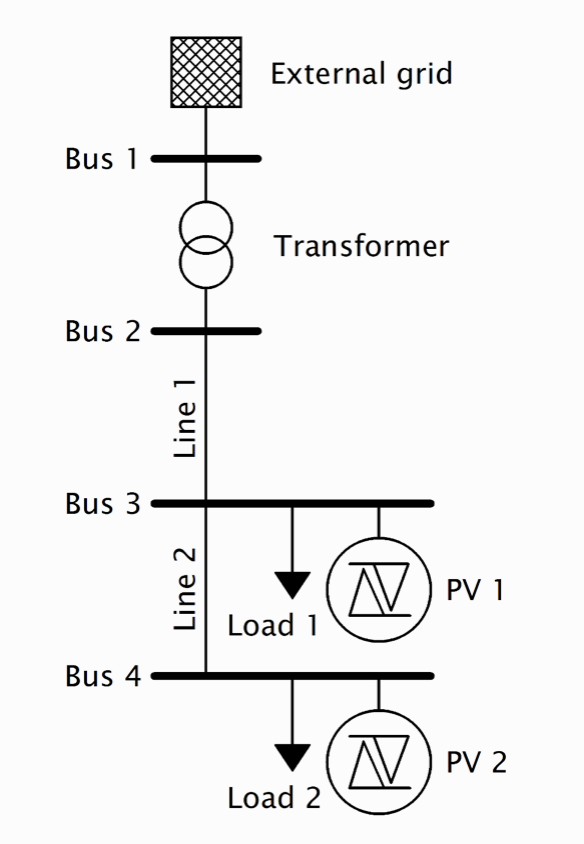
\includegraphics[scale=0.5]{images/four_bus_system.png}
      \caption{four bus system}
      \label{fig.4_bus_system}
    \end{figure}

    Table \ref{tab.Confusion_Matrix_4bus} shows the results. From the table, \ref{tab.Confusion_Matrix_4bus} it can be seen that the proposed method can predict perfectly location of invisible solar PV.
    \begin{table}[H]
      \centering
      \caption{Results of invisible solar PV identification on 4 bus system}
      \begin{tabular}{cc|c|c|}
        \cline{3-4}
                                                                                                                &     & \multicolumn{2}{l|}{Actual PV located} \\ \cline{3-4}
                                                                                                                &     & Yes                & No                \\ \hline
        \multicolumn{1}{|l|}{\multirow{2}{*}{\begin{tabular}[c]{@{}l@{}}Prediction \\ PV located\end{tabular}}} & Yes & 126                & 0                \\ \cline{2-4}
        \multicolumn{1}{|l|}{}                                                                                  & No  & 9                  & 60                \\ \hline
      \end{tabular}
      \label{tab.Confusion_Matrix_4bus}
    \end{table}
    The results is tested by $\text{F}_{1}$ score and MCC using Equation~\ref{eq.F_1_score}, \ref{eq.MCC}.
    The $\text{F}_{1}$ score is 0.965. The MCC is 0.901
    The false negative (FN) occurs when invisible solar PV's capacity is 1-2 kW where maximum demand is around 30 kW.

    \begin{table}[H]
      \centering
      \caption{Results of invisible solar PV estimation on 4 bus system}
      \begin{tabular}{ccc}
        \hline
        Size of invisible solar PV (kW) & MAE(kW) & MAPE (\%) \\
        \hline
        1-10                  & 0.77            & 13.9            \\
        11-20                 & 2.4             & 16.9            \\
        21-30                 & 3.75            & 14.2            \\
        31-40                 & 4.42            & 12              \\
        41-50                 & 3.85            & 8.4\\
        \hline
      \end{tabular}
      \label{tab.Error_4bus}
    \end{table}
    The overall MAPE is 13.587 \% and MAE is 2.919 kW.



  \subsection{CIGRE system}

    \begin{figure}[H]
      \center
      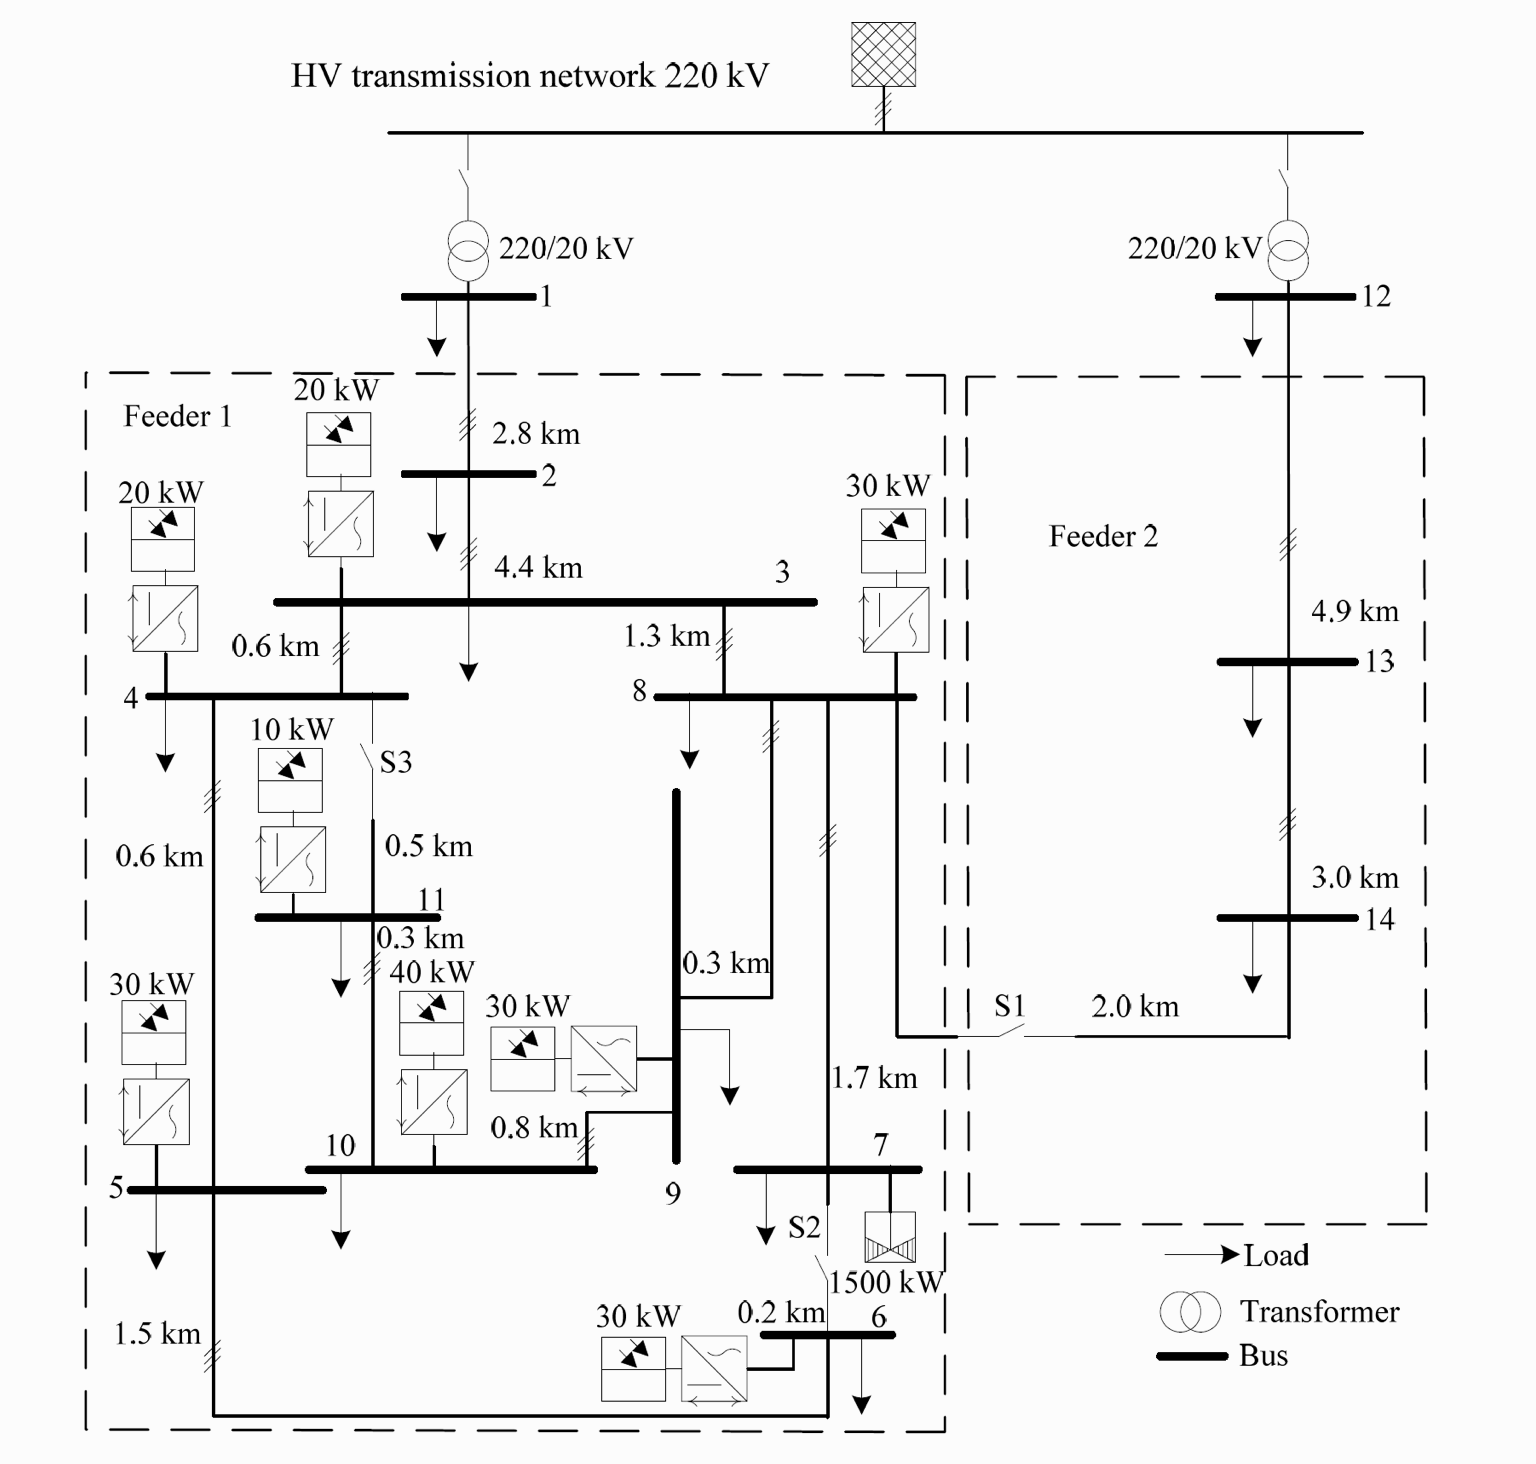
\includegraphics[scale=0.25]{images/CIGRE_network.png}
      \caption{CIGRE network}
      \label{fig.CIGRE_network}
    \end{figure}

    Table \ref{tab.Confusion_Matrix_CIGRE} shows the results. From the table, \ref{tab.Confusion_Matrix_4bus} it can be seen that the proposed method can predict perfectly location of invisible solar PV.

    \begin{table}[H]
      \centering
      \caption{Results of invisible solar PV identification on CIGREsystem}
      \begin{tabular}{cc|c|c|}
        \cline{3-4}
                                                                                                                &     & \multicolumn{2}{l|}{Actual PV located} \\ \cline{3-4}
                                                                                                                &     & Yes                & No                \\ \hline
        \multicolumn{1}{|l|}{\multirow{2}{*}{\begin{tabular}[c]{@{}l@{}}Prediction \\ PV located\end{tabular}}} & Yes & 154                & 8                 \\ \cline{2-4}
        \multicolumn{1}{|l|}{}                                                                                  & No  & 3                  & 159                \\ \hline
      \end{tabular}
      \label{tab.Confusion_Matrix_CIGRE}
    \end{table}

    The results is tested by $\text{F}_{1}$ score and MCC using Equation~\ref{eq.F_1_score}, \ref{eq.MCC}.
    The $\text{F}_{1}$ score is 0.965. The MCC is 0.9325.
    The false negative (FN) occurs when invisible solar PV's capacity is 10-20 kW.

    \begin{table}[H]
      \centering
      \caption{Results of invisible solar PV estimation on CIGRE system}
      \begin{tabular}{ccc}
        \hline
        Size of invisible solar PV (kW) & MAE (kW) & MAPE (\%) \\
        \hline

        1-100                  & 9.01            & 17.60            \\
        101-200                 & 24.3            & 15.97            \\
        201-300                & 50.00            & 19.85            \\
        301-400               & 52.55            & 13.98             \\
        401-500              & 54.92            & 12.28 \\
        \hline

      \end{tabular}
      \label{tab.Error_CIGRE}
    \end{table}

    The overall MAPE is 16.27 \% and MAE is 37.58 kW.
